\documentclass{article}

\usepackage[english,ngerman]{babel}
\usepackage[a3paper, landscape, margin=1.5cm]{geometry}
\usepackage{fancyhdr}
\usepackage{graphicx}
\usepackage{xcolor}
\usepackage{listings}
\usepackage{xcolor-solarized}
\usepackage{tikz}
\usepackage{caption}
\usepackage{titlesec}
\usepackage{multicol}
\usepackage{amssymb}

\setlength{\columnsep}{1cm}
\setlength{\headheight}{35pt}

\pagestyle{fancy}
\fancyhf{}
\lhead{Jonas Mohr, MC2}
\chead{Externer Versuch: Do it yourself - Experiment}
\rhead{
\includegraphics[height=10mm]{../images/Logo.png}}

\definecolor{NavyBlue}{RGB}{16, 5, 237}
\definecolor{BurntOrange}{RGB}{237, 82, 5}
\definecolor{NavyBlue}{RGB}{0,0,255}

\lstdefinelanguage{Kotlin}{
  comment=[l]{//},
  commentstyle={\color{gray}\ttfamily},
  emph={filter, first, firstOrNull, forEach, lazy, map, mapNotNull, println, ascending},
  emphstyle={\solarized@base03},
  identifierstyle=\color{black},
  keywords={!in, !is, abstract, actual, annotation, as, as?, break, by, catch, class, companion, const, constructor, continue, crossinline, data, delegate, do, dynamic, else, enum, expect, external, false, field, file, final, finally, for, fun, get, if, import, in, infix, init, inline, inner, interface, internal, is, lateinit, noinline, null, object, open, operator, out, override, package, param, private, property, protected, public, receiveris, reified, return, return@, sealed, set, setparam, super, suspend, tailrec, this, throw, true, try, typealias, typeof, val, var, vararg, when, where, while},
  keywordstyle={\color{violet}\bfseries},
  morecomment=[s]{/*}{*/},
  morestring=[b]",
  morestring=[s]{"""*}{*"""},
  ndkeywords={ValuePattern, ValuePatternPart, ValueRelationType, @Deprecated, @JvmField, @JvmName, @JvmOverloads, @JvmStatic, @JvmSynthetic, Array, Byte, Double, Float, Int, Integer, Iterable, Long, Runnable, Short, String, Any, Unit, Nothing},
  ndkeywordstyle={\color{cyan}\bfseries},
  sensitive=true,
  stringstyle={\color{base3}\ttfamily},
  basicstyle=\small,
}

\begin{document}
\begin{center}
   \Large\textbf{Automatisierte Verkehrsbeobachtung mithilfe eines Beschleunigungssensors}
\end{center}
\begin{multicols*}{3}
   \section*{Vorgehen}
   Mithilfe der \emph{Phyphox}-App wird die Beschleunigung in x, y und z-Richtung während einer Autofahrt aufgenommen.\\
   Anschließend werden die aufgenommen Daten vollautomatisiert ausgewertet.
   \begin{center}
      \captionsetup{justification=centering}
      \begin{tikzpicture}
         \draw (0, 0) rectangle ++(1, 2);
         \draw (0.1, 1.3) rectangle ++(0.8, 0.3);
         \draw (0, 1.2) to (1, 1.2);
         \draw (0, 0.5) to (1, 0.5);
         \draw[color=blue][->][thick] (0.5, 1) to (0.5, 2.5);
         \node[color=blue] (Y) at (0.5, 2.7) {$y$};
         \draw[color=green][->][thick] (0.5, 1) to (2, 1);
         \node[color=green] (X) at (2.2, 1) {$x$};
         \draw[color=red][fill=red] (0.5, 1) ellipse (0.1 and 0.1);
         \node[color=red] (Z) at (0.2, 0.8) {$z$};
      \end{tikzpicture}
      \captionof{figure}{Sensor Ausrichtung im Auto}
      \label{fig:sensor_alignment}
   \end{center}
   \section*{Auswertung}
   Die Auswertung erfolgt über eine selbst entwickelte Anwendung. Zu Beginn werden die Daten im CSV-Format (Comma separated value) eingelesen.\\
   Anschließend werden die Rohdaten in sog. \emph{ValueRelation}s überführt. Dabei handelt es sich um Beziehungen zwischen zwei aufeinanderfolgende Werte aus Phyphox.
   Diese Relationen enthalten Daten, etwa die zwei originalen Werte, die Differenz deren und ob der Wert ansteigt, abfällt oder gleich bleibt.\\
   \begin{center}
      \captionsetup{justification=centering}
      \begin{tabular}{ |c | c | c | c | c | c | }
         \hline
         relation & first & second & diff & firstTime & secondTime \\
         \hline
         ASC      & 0.5   & 1.2    & 0.7  & 0.02      & 0.05       \\
         \hline
      \end{tabular}
      \captionof{figure}{Beispielhafte ValueRelation}
      \label{fig:sample_ValueRelation}
   \end{center}
   Nun werden in den Datensätzen bestimmte vordefinierte Muster gesucht, beispielsweise:\\
   \begin{lstlisting}[language=Kotlin]
ValuePattern(
   ValuePatternPart(
      ValueRelationType.ASCENDING,
      2,
      Int.MAX_VALUE,
      0.5,
      Double.MAX_VALUE
   ), ...
)
        \end{lstlisting}
   In diesem Beispiel wird ein Muster definiert, welches zwischen $2$ und $2147483647$ (Int.MAX\_VALUE) ansteigende Datenpunkte
   mit einer Steigung zwischen $0.5$ und $1.7*10^{308}$ (Double.MAX\_VALUE) akzeptiert.\\
   \begin{center}
      \captionsetup{justification=centering}
      \begin{tikzpicture}
         \draw[dotted] (-3.1,-2.1) grid (3.1,2.1);
         \draw[color=red] (-3,-2) to  (3,2);
         \draw[color=blue] (-2, -2) to (3, 2);
         \draw[color=green] (-3,-2) to (-1, 0) to (0,0.5) to (1,2);
      \end{tikzpicture}
      \captionof{figure}{Beispielhafte Verläufe, welche vom obigen Muster akzeptiert werden}
      \label{fig:sample_graphs}
   \end{center}
   \vfill\null
   \columnbreak
   \section*{Ergebnisse}
   Die hier betrachtete Autofahrt dauerte $\thicksim$ 18 Minuten.\\
   Die Rohdaten sehen wie folgt aus:\\
   \begin{center}
      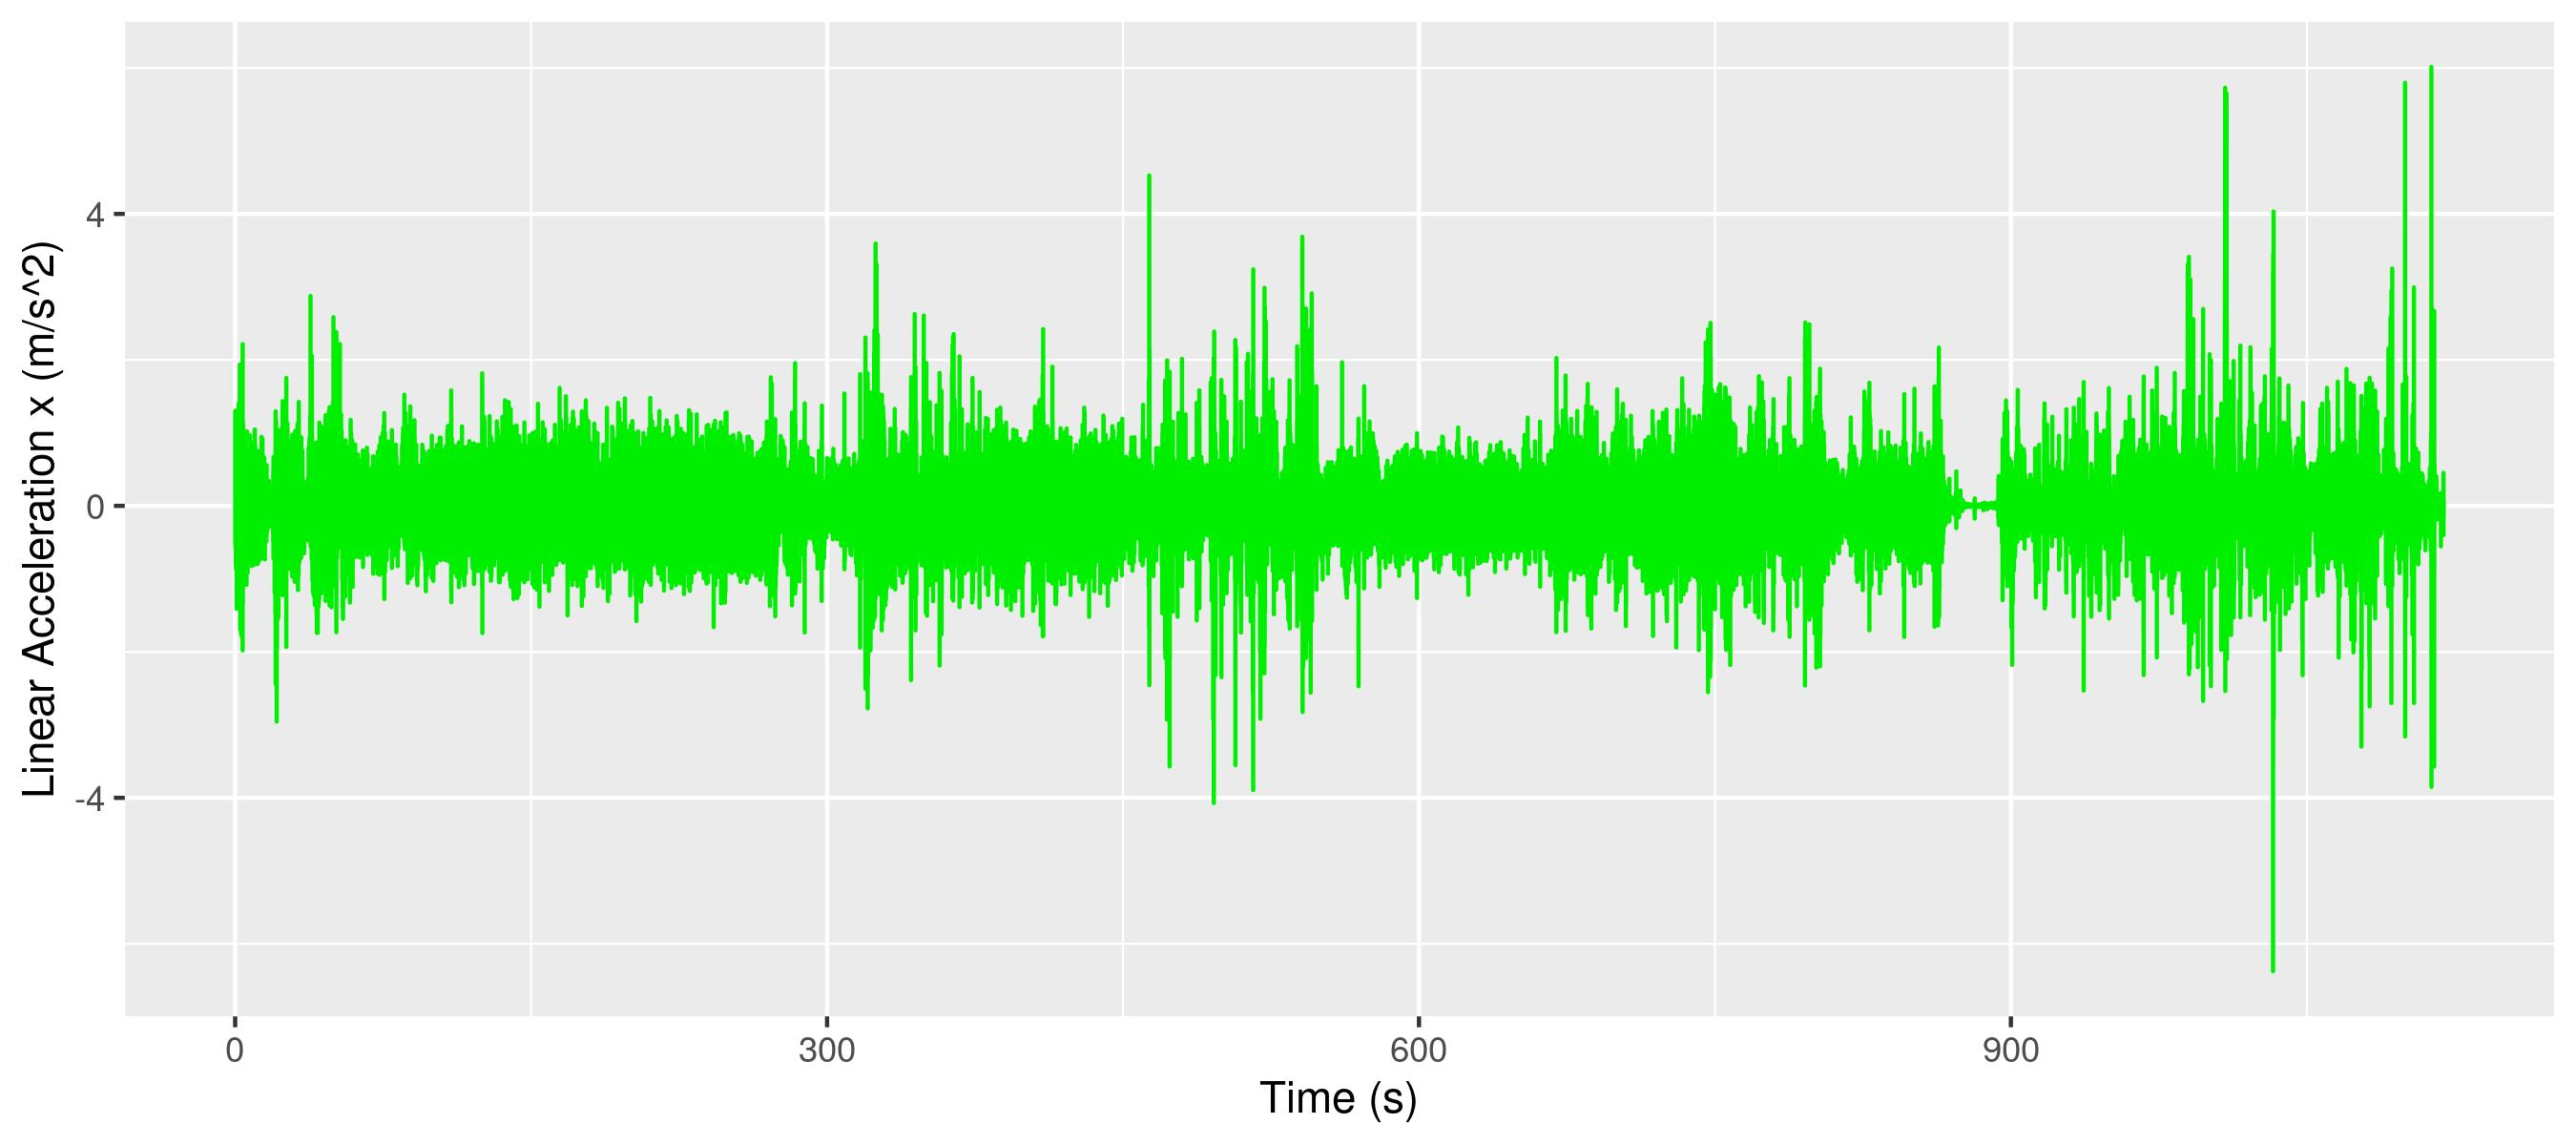
\includegraphics[width=0.9\linewidth]{../images/Calculations_cell_2_output_0}
      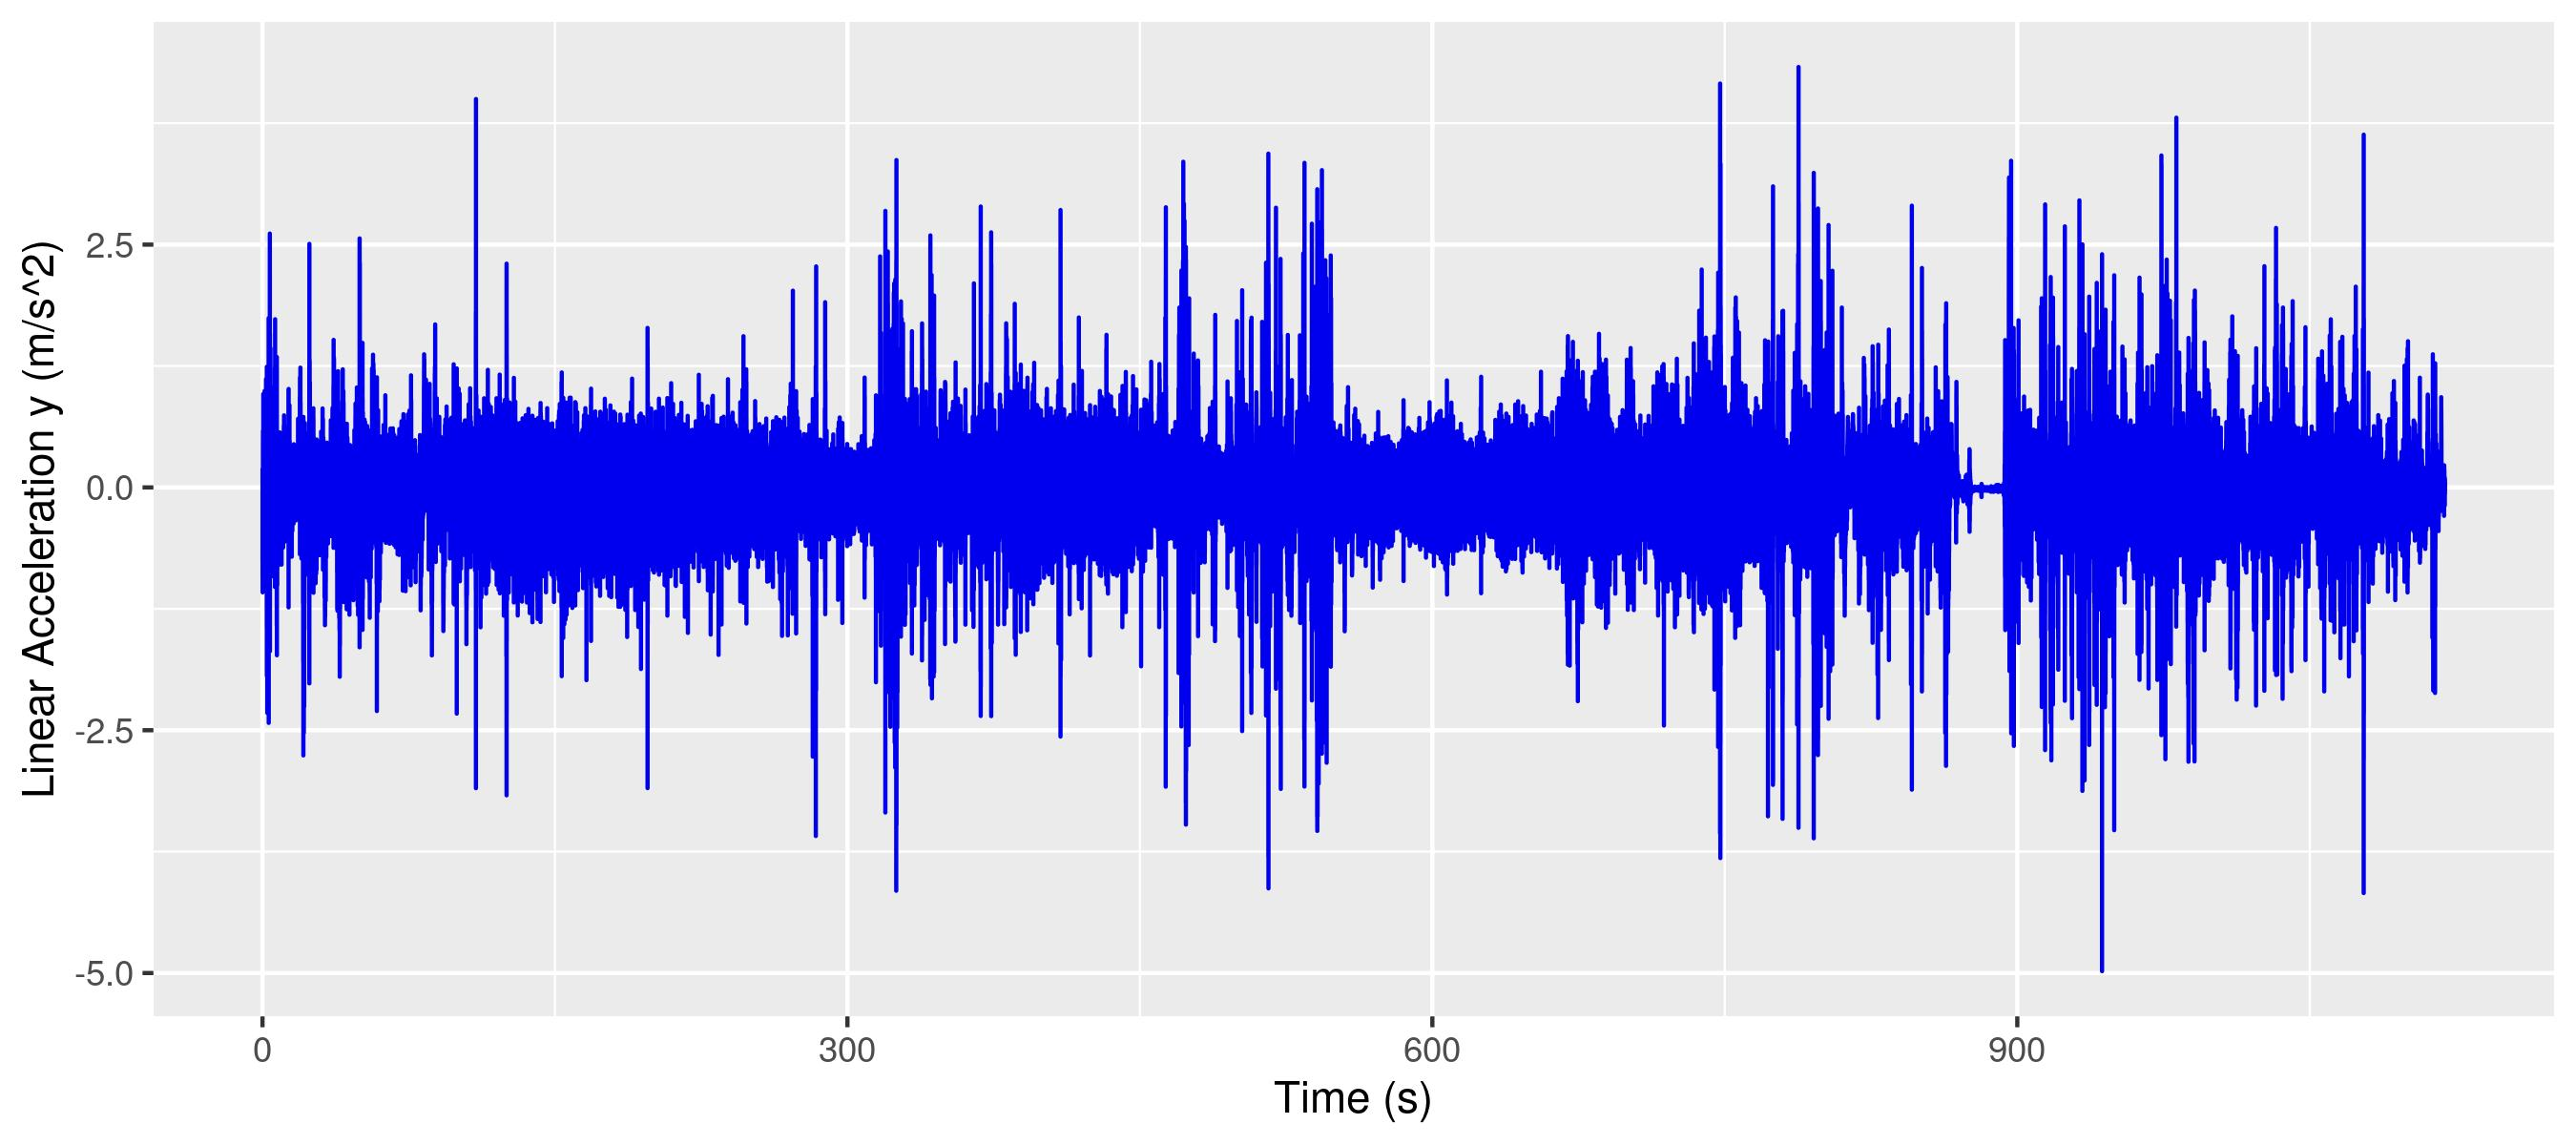
\includegraphics[width=0.9\linewidth]{../images/Calculations_cell_3_output_0}
      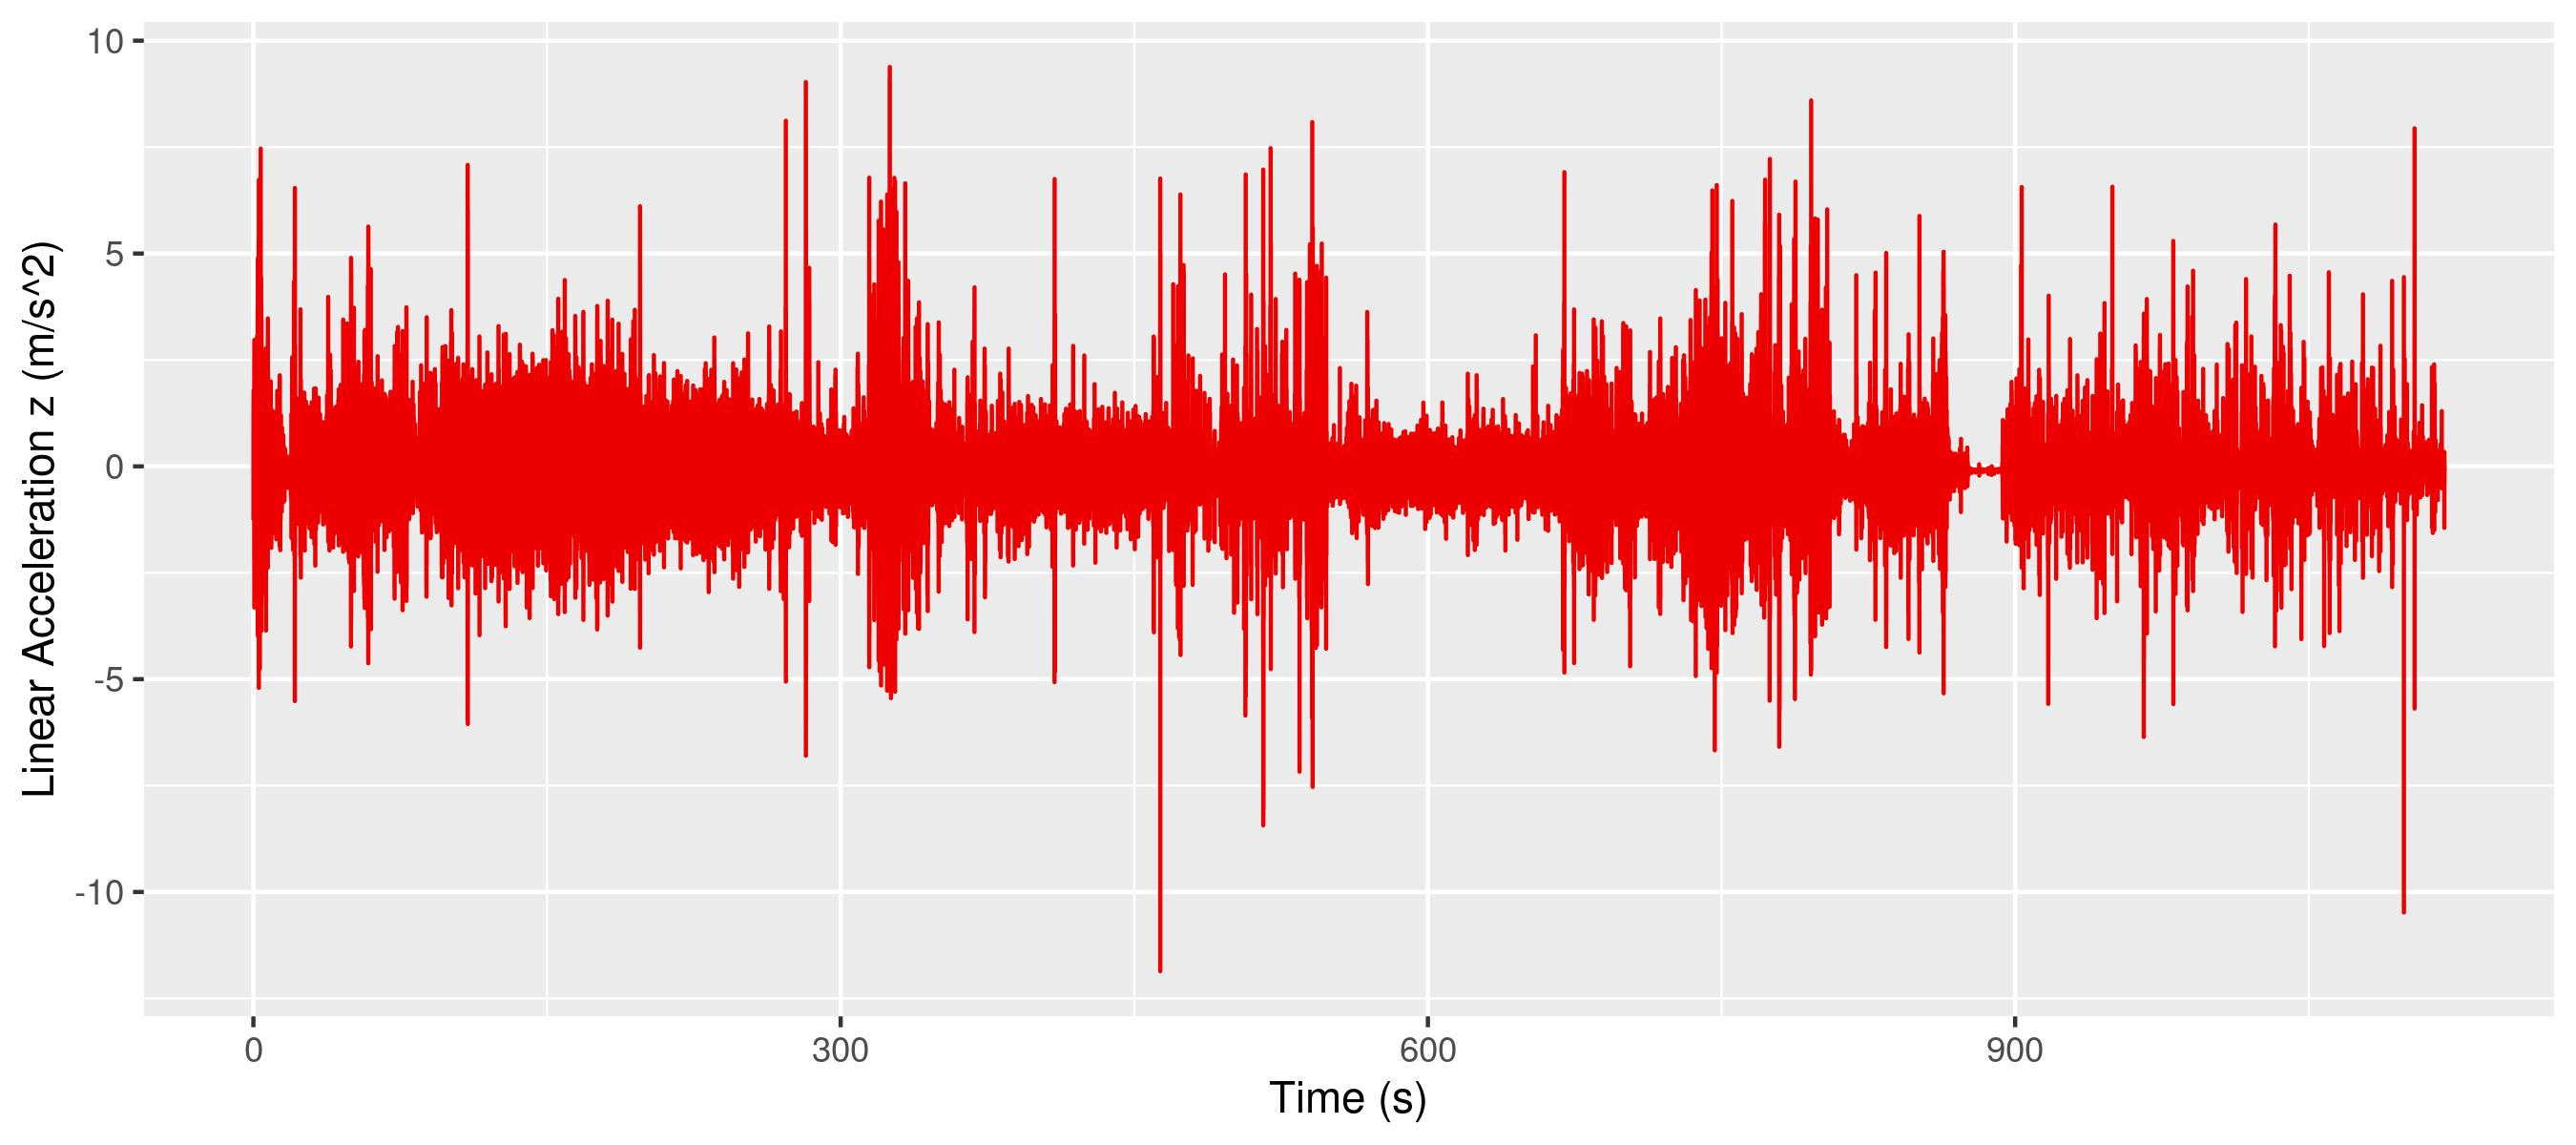
\includegraphics[width=0.9\linewidth]{../images/Calculations_cell_4_output_0}
   \end{center}
   \subsection*{Kurvenerkennung}
   Um Kurven zu erkennen wird die Beschleunigung in x-Richtung betrachtete. Nach Anwendung des passenden Musters ergibt sich foldendes Bild:
   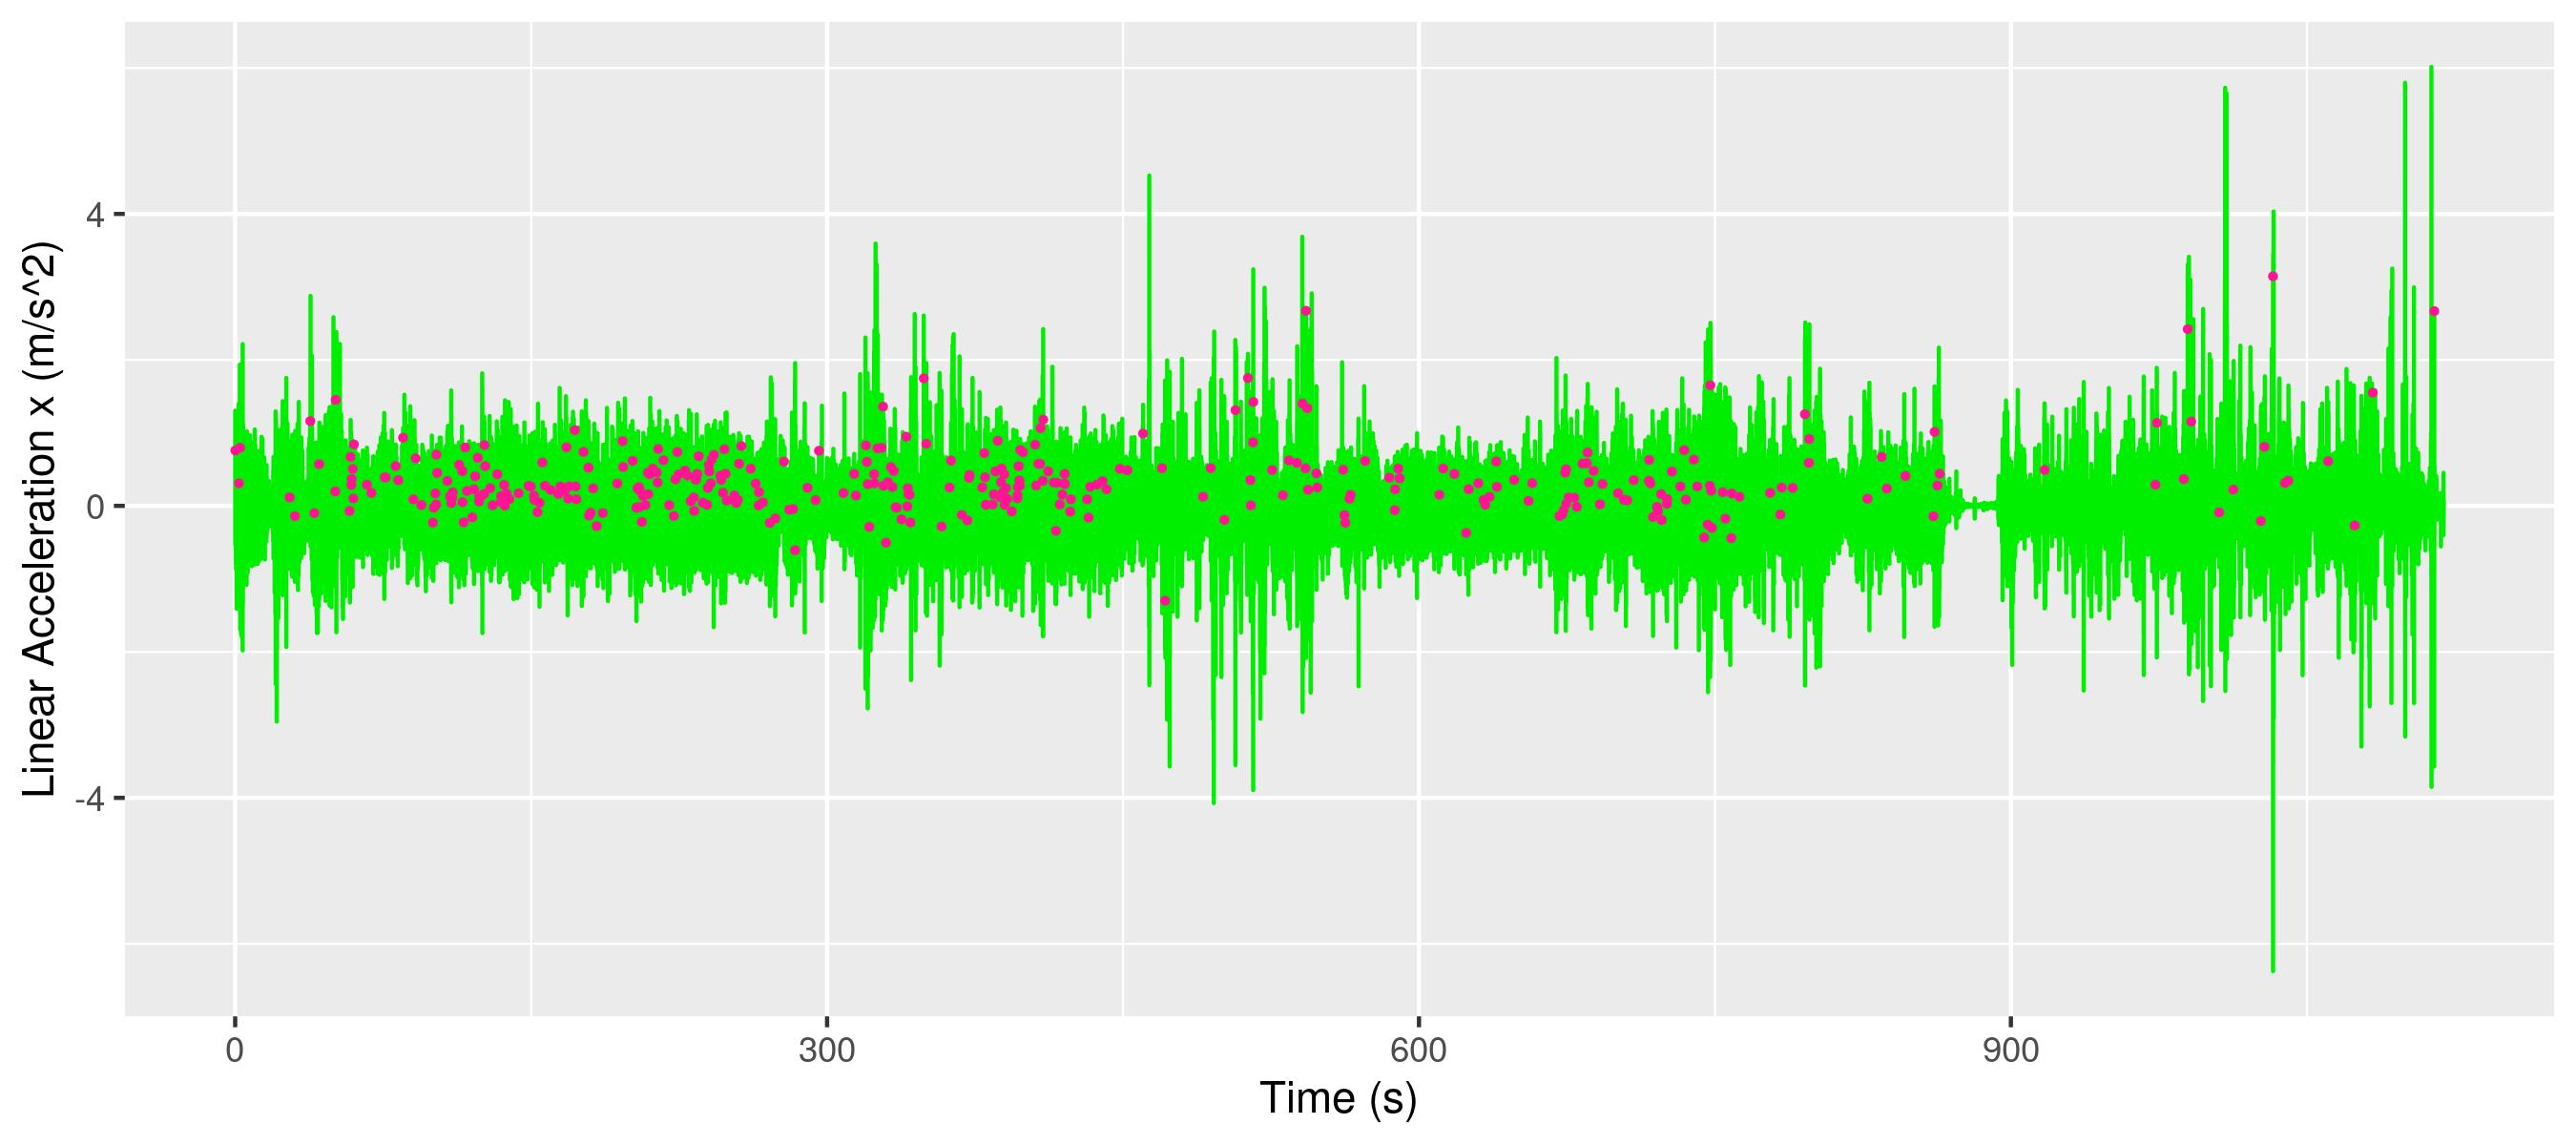
\includegraphics[width=\linewidth]{../images/Calculations_cell_7_output_0}
   Hier entspricht jeder Punkt einer Kurve.
   \vfill\null
   \columnbreak
   \subsection*{Erkennung starke Beschleunigen / starkes Abbremsen}
   Um ein starkes Beschleunigen / Abbremsen festzustellen werden die Daten in y-Richtung betrachtet. Dabei wird nach kurzen, starken Ausschlägen gefiltert:
   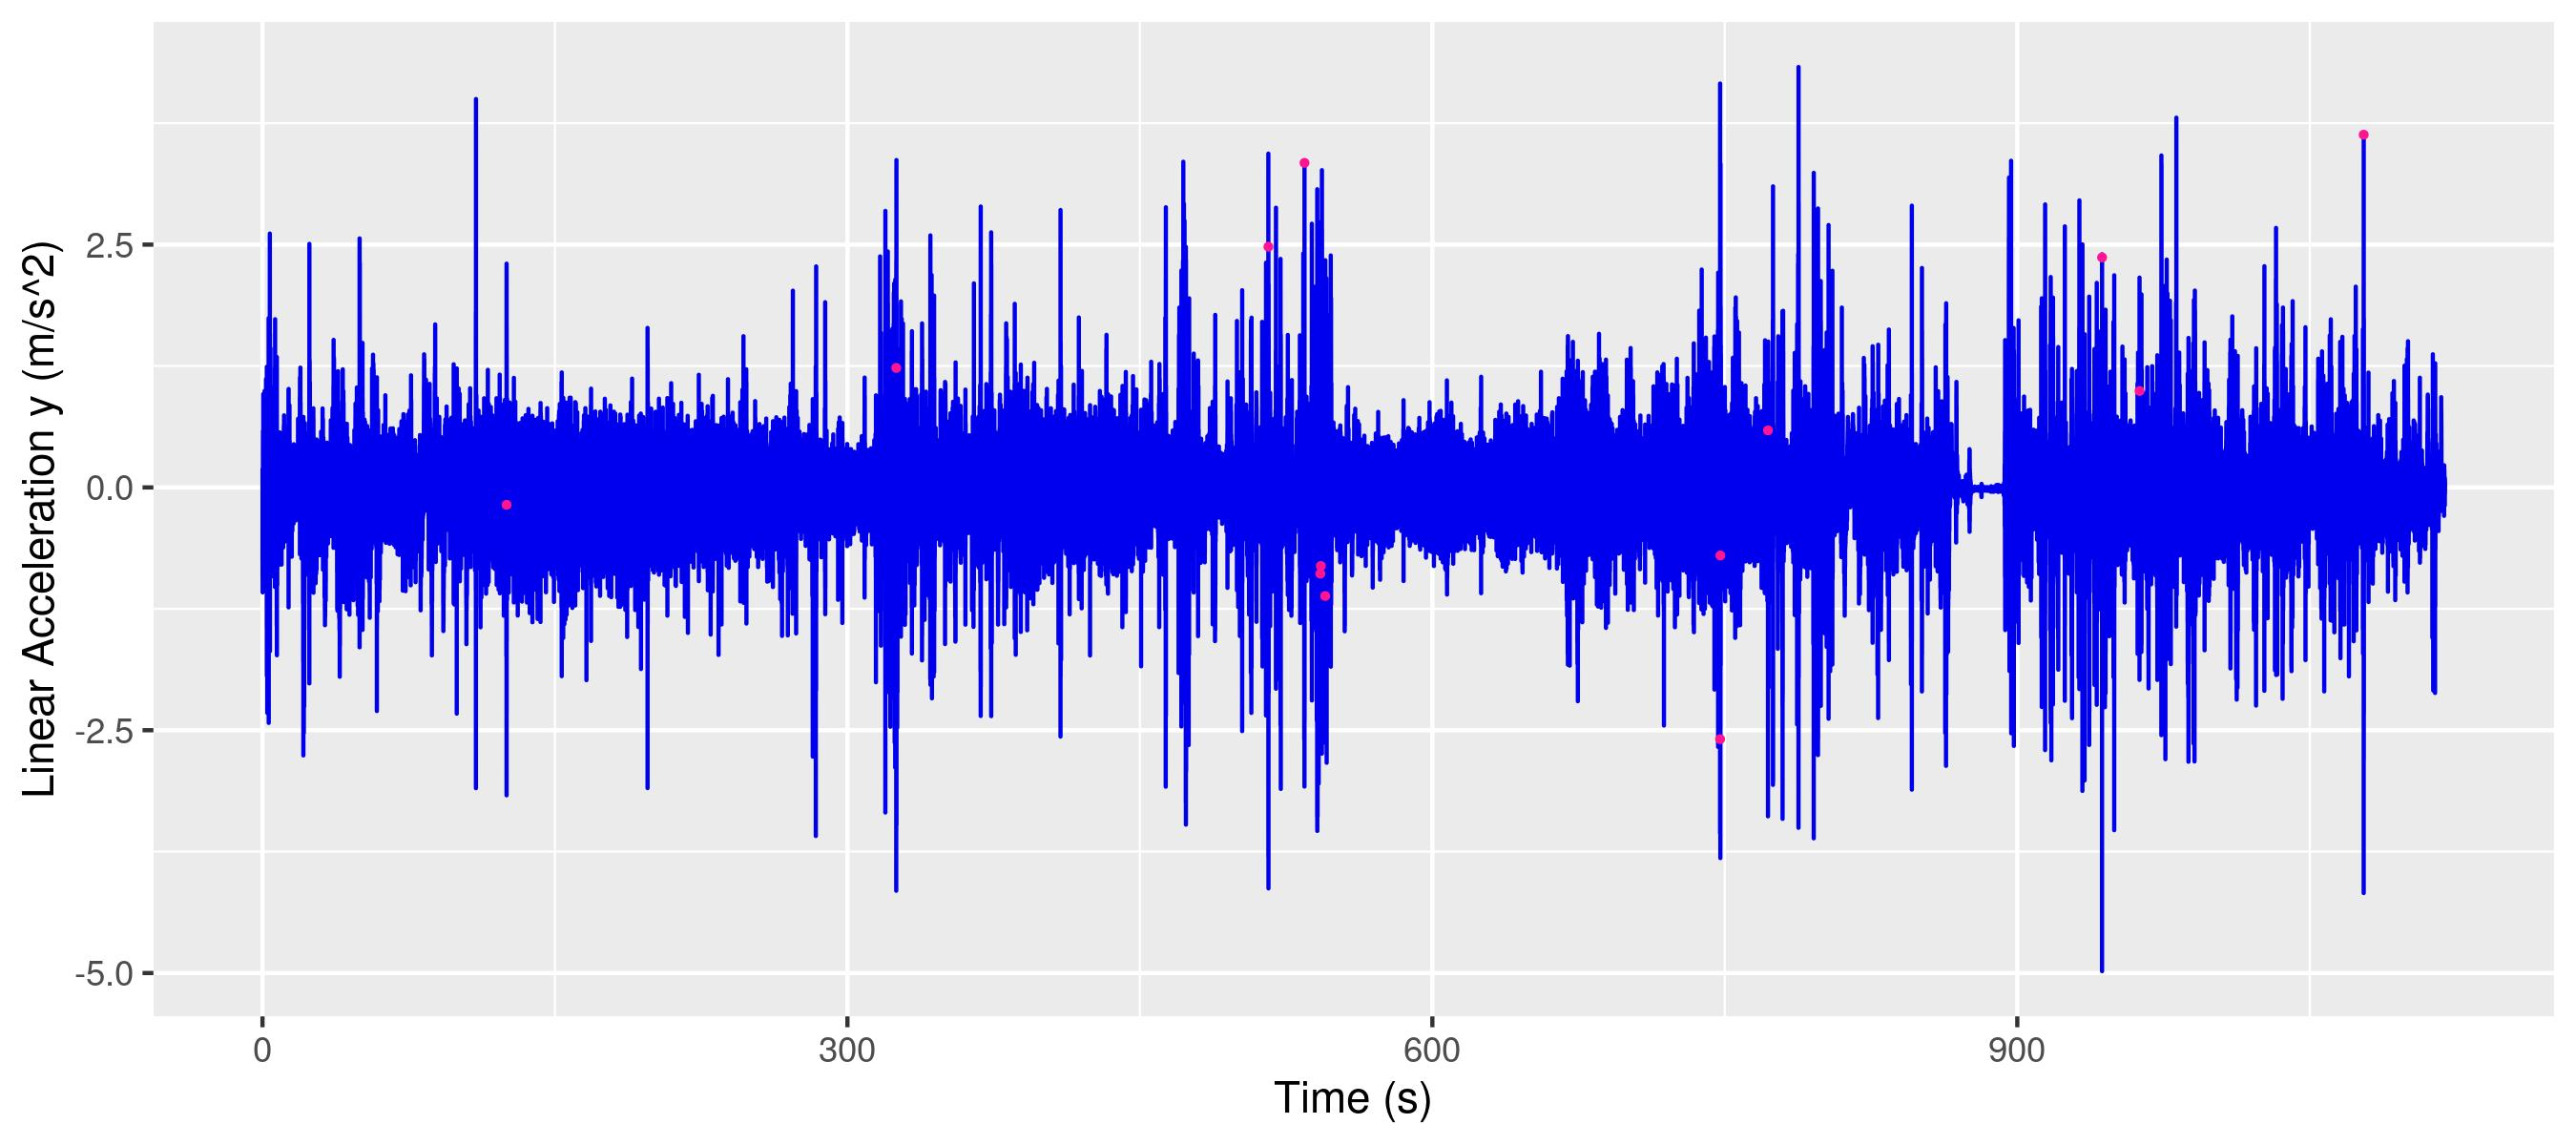
\includegraphics[width=\linewidth]{../images/Calculations_cell_8_output_0}
   Jeder Punkt hier entspricht einer Beschleunigung / einem Bremsen\\ von $<=4m/s^{2}$
   \section*{Technisches}
   Die Software ist in \emph{Kotlin} realisiert, einer Java-ähnlichen Sprache, die auch auf der \emph{JVM} (Java Virtual Machine) läuft.\\
   Also Buildsystem dient \emph{Make} und \emph{Maven}. \\
   Zum einlesen und verarbeiten der Rohdaten dient die Library \emph{krangl}, zur Visualisierung \emph{kravis}\\
   Also Frontend für die Daten dient \emph{Jupyter notebook} mit dem \emph{Kotlin kernel}. \\
   Als IDE kommt \emph{IntelliJ Ultimate} zum Einsatz.\\
   \emph{Git} wurde zur Versionsverwaltung verwendet.\\
   Das Plakat wurde in \emph{\LaTeX} erstellt.\\
   Alle Diagramme wurden aus \emph{Jupyter notebook} exportiert.\\
   Bilder wurden mit \emph{Tikz} gezeichnet.\\
   Das volle Projekt inklusiv Rohdaten, Sourcecode für das Programm und Poster und Bilder sind unter https://github.com/MohrJonas/DIYPhysicsExperiment verfügbar:\\
   \vspace*{3px}
   \begin{center}
      \captionsetup{justification=centering}
      
\includegraphics[scale=0.3]{../images/qr_code}
      \captionof{figure}{Scannbarer QR-Code}
      \label{fig:qr_code}
   \end{center}
\end{multicols*}
\end{document}